\section{Theorie}
\label{sec:Theorie}
Brückenschaltungen werden in der Messtechnik 
eingesetzt um die Auflösung einer Messung zu erhöhen
oder eine pysikalische Größe,
die sich als elektrischer Widerstand darstellen lässt,
zu bestimmen. \\
\\
Dafür muss eine Abgleichbedingung der
Brückenschaltung erfüllt sein. Generell benötigt eine
Brückenschaltung eine Speisespannung $U_S$, den zu
ermittelnden elektrischen Widerstand und bekannte
elektrische Bauteile um ein Widerstandsverhältnis
zu bestimmen.
Die Abgleichbedingung besteht darin, dass die
Brückenspannung $U_{Br}$ zwischen zwei Punkten
verschwindet.

\begin{figure}[H]
\centering
    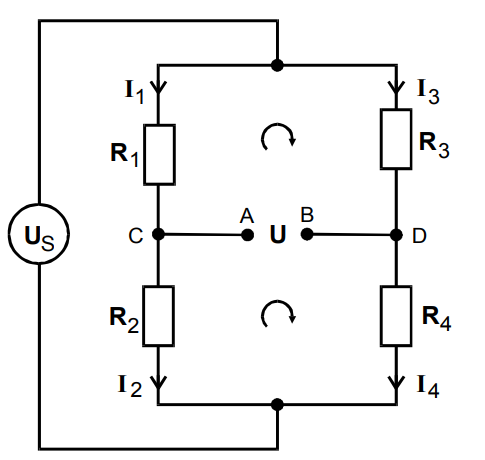
\includegraphics[height= 5cm]{content/Allgemein.png}
    \caption{Allgemeine Funktionsweise einer Brückenschaltung\cite[216]{sample}}
\end{figure}

\noindent Ist die Abgleichbedingung erfüllt kann
aus dem Widerstandsverhältnis der
unbekannte Widerstand bestimmt werden.\\
\\
Dieses Verhältnis ergibt sich aus den beiden
Kirchhoffschen Gesetzen
\begin{equation}
   \sum_{k} I_k =0
\end{equation}
\begin{equation}
    \sum_{k} U_k =0,
\end{equation}

\noindent die besagen, dass die Summe aller eingehenden
Ströme eienes Knotens gleich der Summe aller ausgehenden
Ströme ist und die Summe aller Spannungen in einer Masche
immer Null ist.
Dadurch lässt sich die Brückenspannung als
\begin{equation}
    U_{Br}=\frac{R_2R_3-R_1R_4}{(R_3+R_4)(R_1+R_4)}U_S
    \label{eq:b}
\end{equation}
\noindent ausdrücken. Sobald $U_{Br}$ verschwindet gilt unabhängig von der
Speisespannung $U_S$
\begin{equation}
    R_2R_3=R_1R_4.
    \label{eq:a}
\end{equation}





\subsection{Wheatstonesche Brücke}
\begin{figure}[H]
\centering
    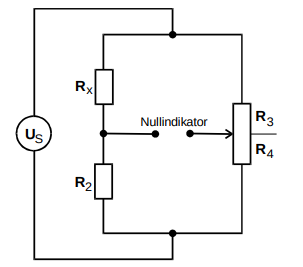
\includegraphics[height= 5cm]{content/Wheatstone.png}
    \caption{Aufbau der Wheatstoneschen Brücke\cite[219]{sample}}
\end{figure}
\noindent Bei der Wheatstoneschen Brücke sind alle
Widerstände Ohmsche Widerstände wobei $R_x$ unbekannt
ist und sich mit Gleichung \ref{eq:a} durch
\begin{equation}
    R_x=R_2\frac{R_3}{R_4}
\end{equation}

\noindent bestimmen lässt. $R_3$ und $R_4$ sind dabei
durch ein Potentiometer realisiert, da zur Berechnung
nur ihr Verhältnis relevant ist.


\subsection{Kapazitätsmessbrücke}
\label{sec:Kap}
\begin{figure}[H]
\centering
    \includegraphics[height= 5cm]{content/Kapazität.png}
    \caption{Aufbau der Kapazitätsmessbrücke\cite[220]{sample}}
\end{figure}
\noindent Mit der Kapazitätsmessbrücke lässt sich eine
unbekannte Kapazität $C_x$ ermitteln. Da es sich
bei einer Kapazität um einen komplexen Widerstand handelt
muss diese Schaltung mit Wechselstrom betrieben werden
Der Innenwiderstand des Kondensators wird durch einen
unbekannten Ohmschen Widerstand $R_x$ ausgedrückt.
Aus Gleichung \ref{eq:a} ergeben dich die zu ermittelnden
Größen als
\begin{equation}
    R_X=R_2\frac{R_3}{R_4}
\end{equation}
\noindent und
\begin{equation}
    C_x=C_2\frac{R_4}{R_3}.
\end{equation}




\subsection{Induktivitätsmessbrücke}
\label{sec:Ind}
\begin{figure}[H]
\centering
    \includegraphics[height= 5cm]{content/Induktivität.png}
    \caption{Aufbau der Induktivitätsmessbrücke\cite[221]{sample}}
\end{figure}
Analog zu \ref{sec:Kap} wird wieder Wechselstrom
verwendet, da es sich bei der zu bestimmenden
unbekannten Induktivität $L_x$ ebenfalls um einen
komplexen Widerstand handelt. Auch hier gibt es einen
unbekannten ohmschen Widerstand $R_x$ der den
inneren Widerstand der Spule darstellt. Ähnlich wie
bei \ref{sec:Kap} lassen sich $R_x$ und $L_x$ mit
Glechung \ref{eq:a} durch
\begin{equation}
    R_x=R_2\frac{R_3}{R_4}
\end{equation}
\noindent und
\begin{equation}
    L_x=L_2\frac{R_3}{R_4}
\end{equation}
\noindent berechnen.



\subsection{Maxwell-Brücke}
\begin{figure}[H]
\centering
    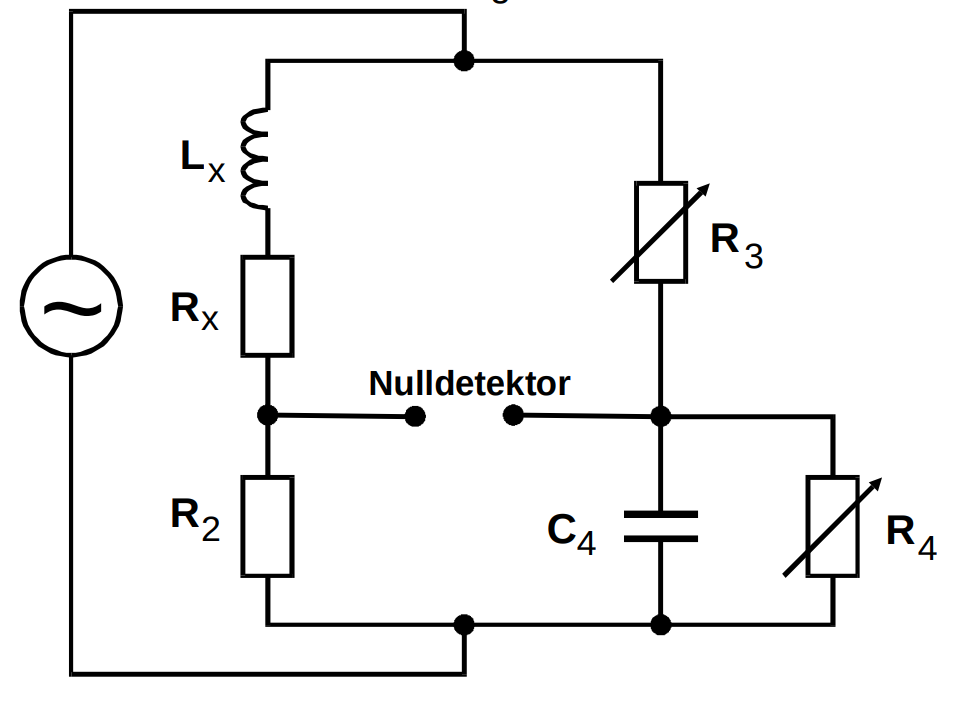
\includegraphics[height= 5cm]{content/Maxwell.png}
    \caption{Aufbau der Maxwell-Brücke\cite[222]{sample}}
\end{figure}

\noindent Diese Schaltung unterscheidet sich von
\ref{sec:Ind} vor allem dadurch, dass zur Bestimmung
der Induktivität $L_x$ keine bereits bekannte
Induktivität nötig ist, sondern nur eine
bekannte Kapazität $C_4$. Der Abgleich ist bei
diesem Aufbau optimal durchführbar wenn
die Wirk- und Blindwiderstände die gleiche
Größenordnung besitzen. $L_x$ und $R_x$ können 
mit Gleichung \ref{eq:a} durch
\begin{equation}
    R_x=R_2\frac{R_3}{R_4}
\end{equation}
\noindent und
\begin{equation}
    L_x=R_2R_3C_4
\end{equation}
\noindent berechnen.



\subsection{Wien-Robinson-Brücke}
\begin{figure}[H]
\centering
    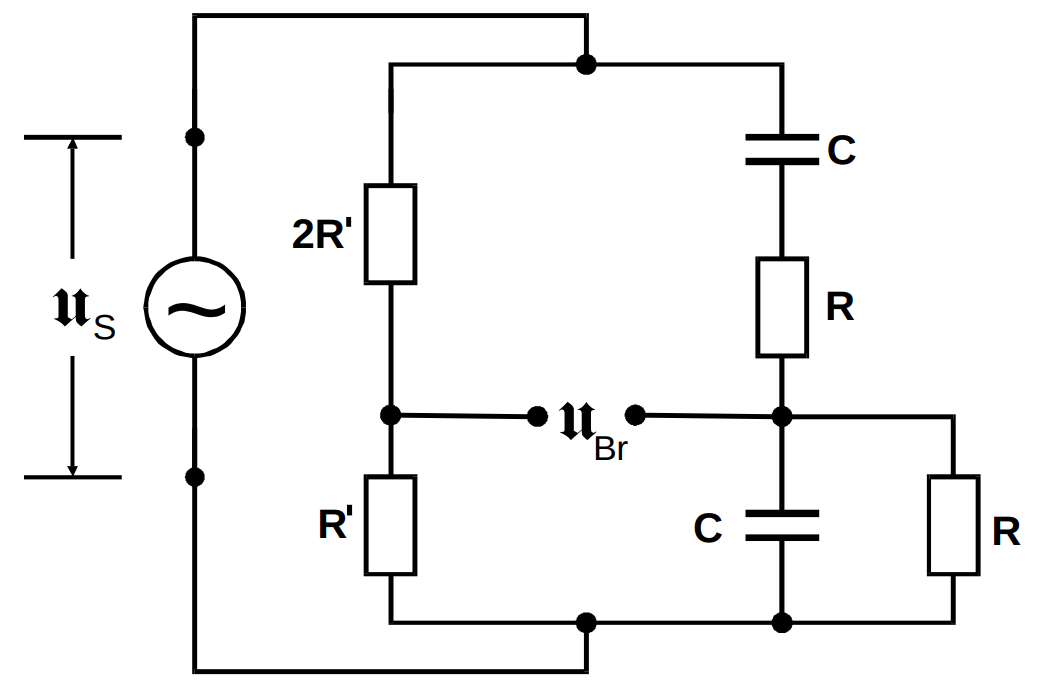
\includegraphics[height= 5cm]{content/Wien-Robinson.png}
    \caption{Aufbau der Wien-Robinson-Brücke\cite[223]{sample}}
\end{figure}
\noindent Anders als bei den anderen Schaltungen ist
die Wien-Robinson-Brücke frequenzabhängig. Bei einer
festen Speisespannung $U_S$ hängt das Verhältnis
$\lvert{\frac{U_{Br}}{U_S}}\rvert$
also bei bekannten elektrischen Bauteilen
nur von der Frequenz $v$ der Speisespannung ab.
Aus Gleichung \ref{eq:b} folgt
\begin{equation}
    U_{Br}=\frac{\omega^2R^2C^2-1}{3(1-\omega^2R^2C^2)+9i\omega RC}U_S
\end{equation}
\begin{equation}
    \iff \Big|\frac{U_{Br}}{U_S}\Bigr| ^2=\frac{1}{9}\frac{(\Omega ^2 -1)^2}{(1-\Omega ^2)^2+9\Omega ^2} \qquad \text{mit} \qquad \Omega := \frac{\omega}{\omega_0}.
\end{equation}




\subsection{Fehlerrechnung}
Bei der Auswertung werden die Mittelwerte 
der errechneten Größen durch die Formel
\begin{equation}
    \bar{x}=\frac{1}{N}\sum_{i=1}^N x_i
\end{equation}
berechnet.\\ 
\\
Der Standardfehler des Mittelwerts beerechnet sich durch

 \begin{equation}
     \Delta\bar{x}=\sqrt{\frac{1}{N(N-1)}\sum_{i=1}^N (x_i-\bar{x})}.
 \end{equation}





DENK AN DAS MESSHEFT!!!!